\section{Implementation}

The Implementation section will cover certain topics about how we solved non-trivial implementation tasks. Problems and their solutions will be discussed.

\subsection{Scheduler}

The major problem of implementing a genetic algorithm is the question of how to represent the solutions. The presented genetic algorithm operations can only be applied when a fitting data model was designed. Historically a representation in the form of a fixed-length vector of values is used. The \emph{crossover} operation applied on two candidate solutions would lead to mixing these values with each other. The \emph{mutation} operation on one candidate solution would lead to randomly change values of the vector.

A generic approach to solve this problem is the encoding of the data model to a byte representation. But since we chose AspectJ respectively Java to implement the scheduler we wanted to use the concept of object-orientied programming and all its advantages. Fortunately we had given a reference solution which was implemented in C++ on which we based our implementation.

Instead of using a byte encoding we used a similarity to the vector. The candidate solutions are represented by using a \emph{Map}.

\[Course \mapsto (Room,Time Slot)\]

Every course is mapped to a tuple defined by a room and a time slot. The time slot is the starting time slot of the course [Figure \ref{fig:map}].

\begin{figure}[H]
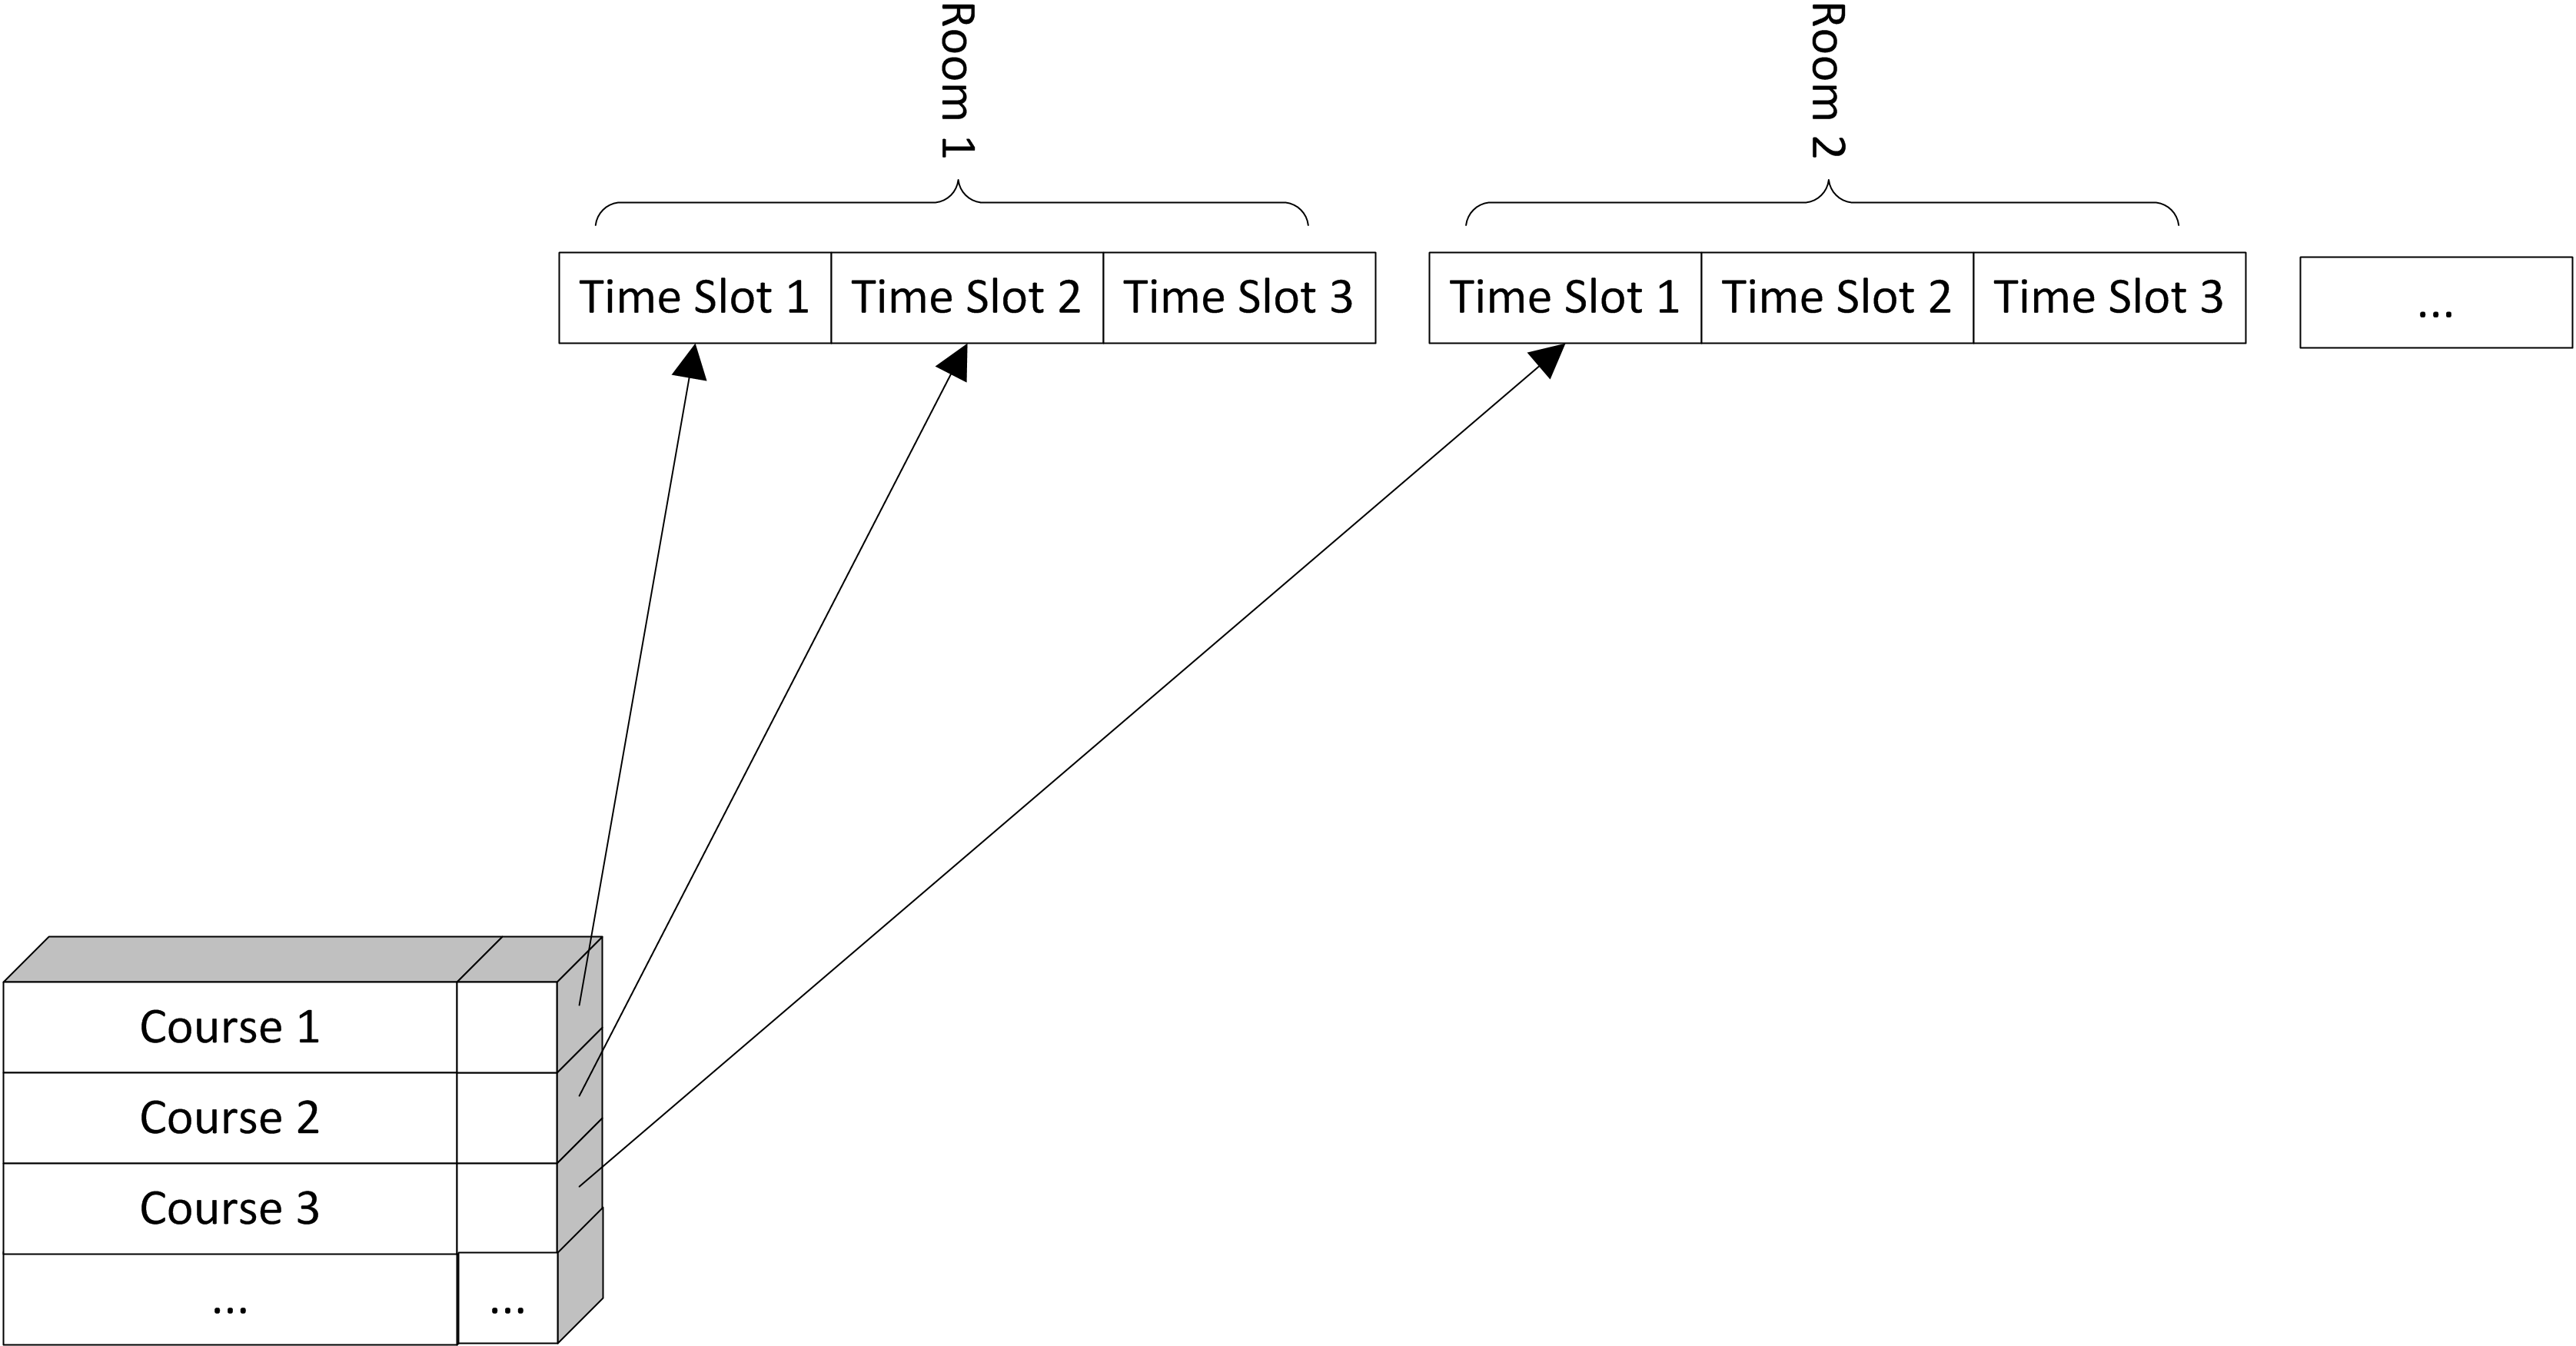
\includegraphics[width=\textwidth]{images/map.png}%
\caption{Every Course is mapped to a tuple defined by a room and a time slot.}%
\label{fig:map}%
\end{figure}

 As a matter of fact this is not sufficient to model the whole candidate solution. Behind this data model lies another data model modeling the whole timetable. The data model is a list of rooms with each having a further list with time slots. On every time slot is another list with courses allocated to this position. A list of courses was chosen because there is the possibility of having one course in the same room at the same time.

\[ [(Room,[(TimeSlot,[Course])] \]

However applying \emph{crossover} and \emph{mutation} takes only affect on the \emph{Map}. An example of executing \emph{crossover} on the designed data model is illustrated in Figure \ref{fig:data-model}.

\begin{figure}[H]
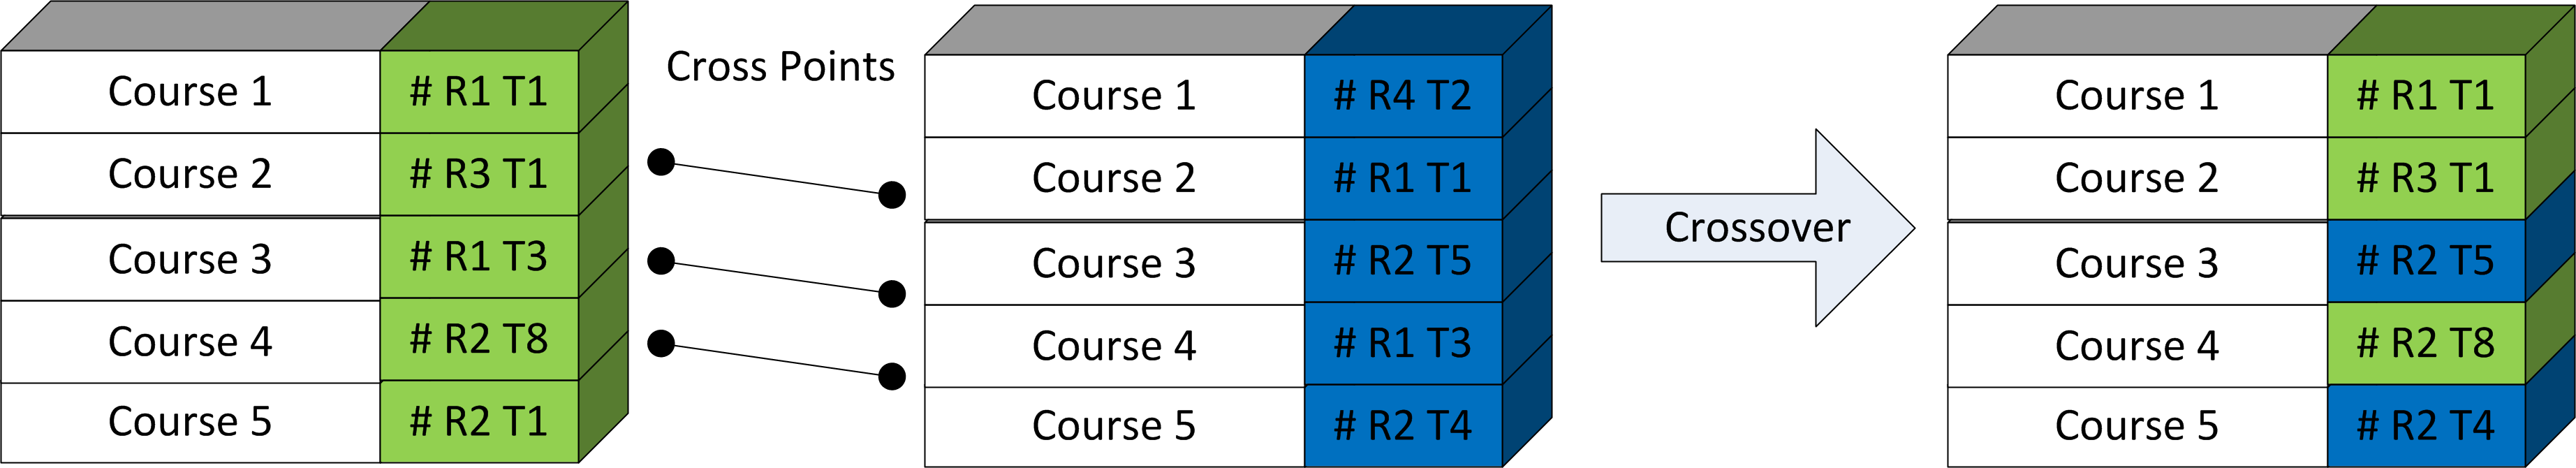
\includegraphics[width=\textwidth]{images/crossover.png}%
\caption{Crossover Operation: A specified amount of cross points is chosen randomly. The courses are iterated and taken over to the offspring candidate solution. When a cross point is met the other candidate solution being crossed over is used to take over its course allocations.}%
\label{fig:data-model}%0
\end{figure}

The scheduler algorithm is a lot about comparing objects. For instance comparing two candidate solutions, comparing two rooms, etc. Therefore we made extensive use of the \emph{java.lang.Comparable} interface of Java. Which in turn made further implementations easier. Because of that a \emph{Sorted List} could be used to keep the best schedules. Every new schedule is inserted into that list and if the list's size succeed $\mu$ the last schedules are dropped. Similiar ease could be realized for the \emph{Greedy Setup} allocation of rooms which are sorted by their features.